\documentclass[../document.tex]{subfiles}
\begin{document}
\chapter{Methodology}
\label{chap: methodology}
We developed a framework to learn traversability directly on ground patches for any robot using purely simulated data. The core idea, originally proposed by Chavez-Garcia et al. \cite{omar2018traversability}, is simple yet elegant, a robot is let travel forward with a fix controller into a simulator on different synthetic terrains. While moving it stores its interactions with the environment, namely pose and orientation. Then we crop a region of ground, a patch, around each traveled position and directly train a neural network on them to predict traversability. Figure \ref{fig : pipeline} shows the framework's steps.

\begin{figure} [htbp]
    \centering
        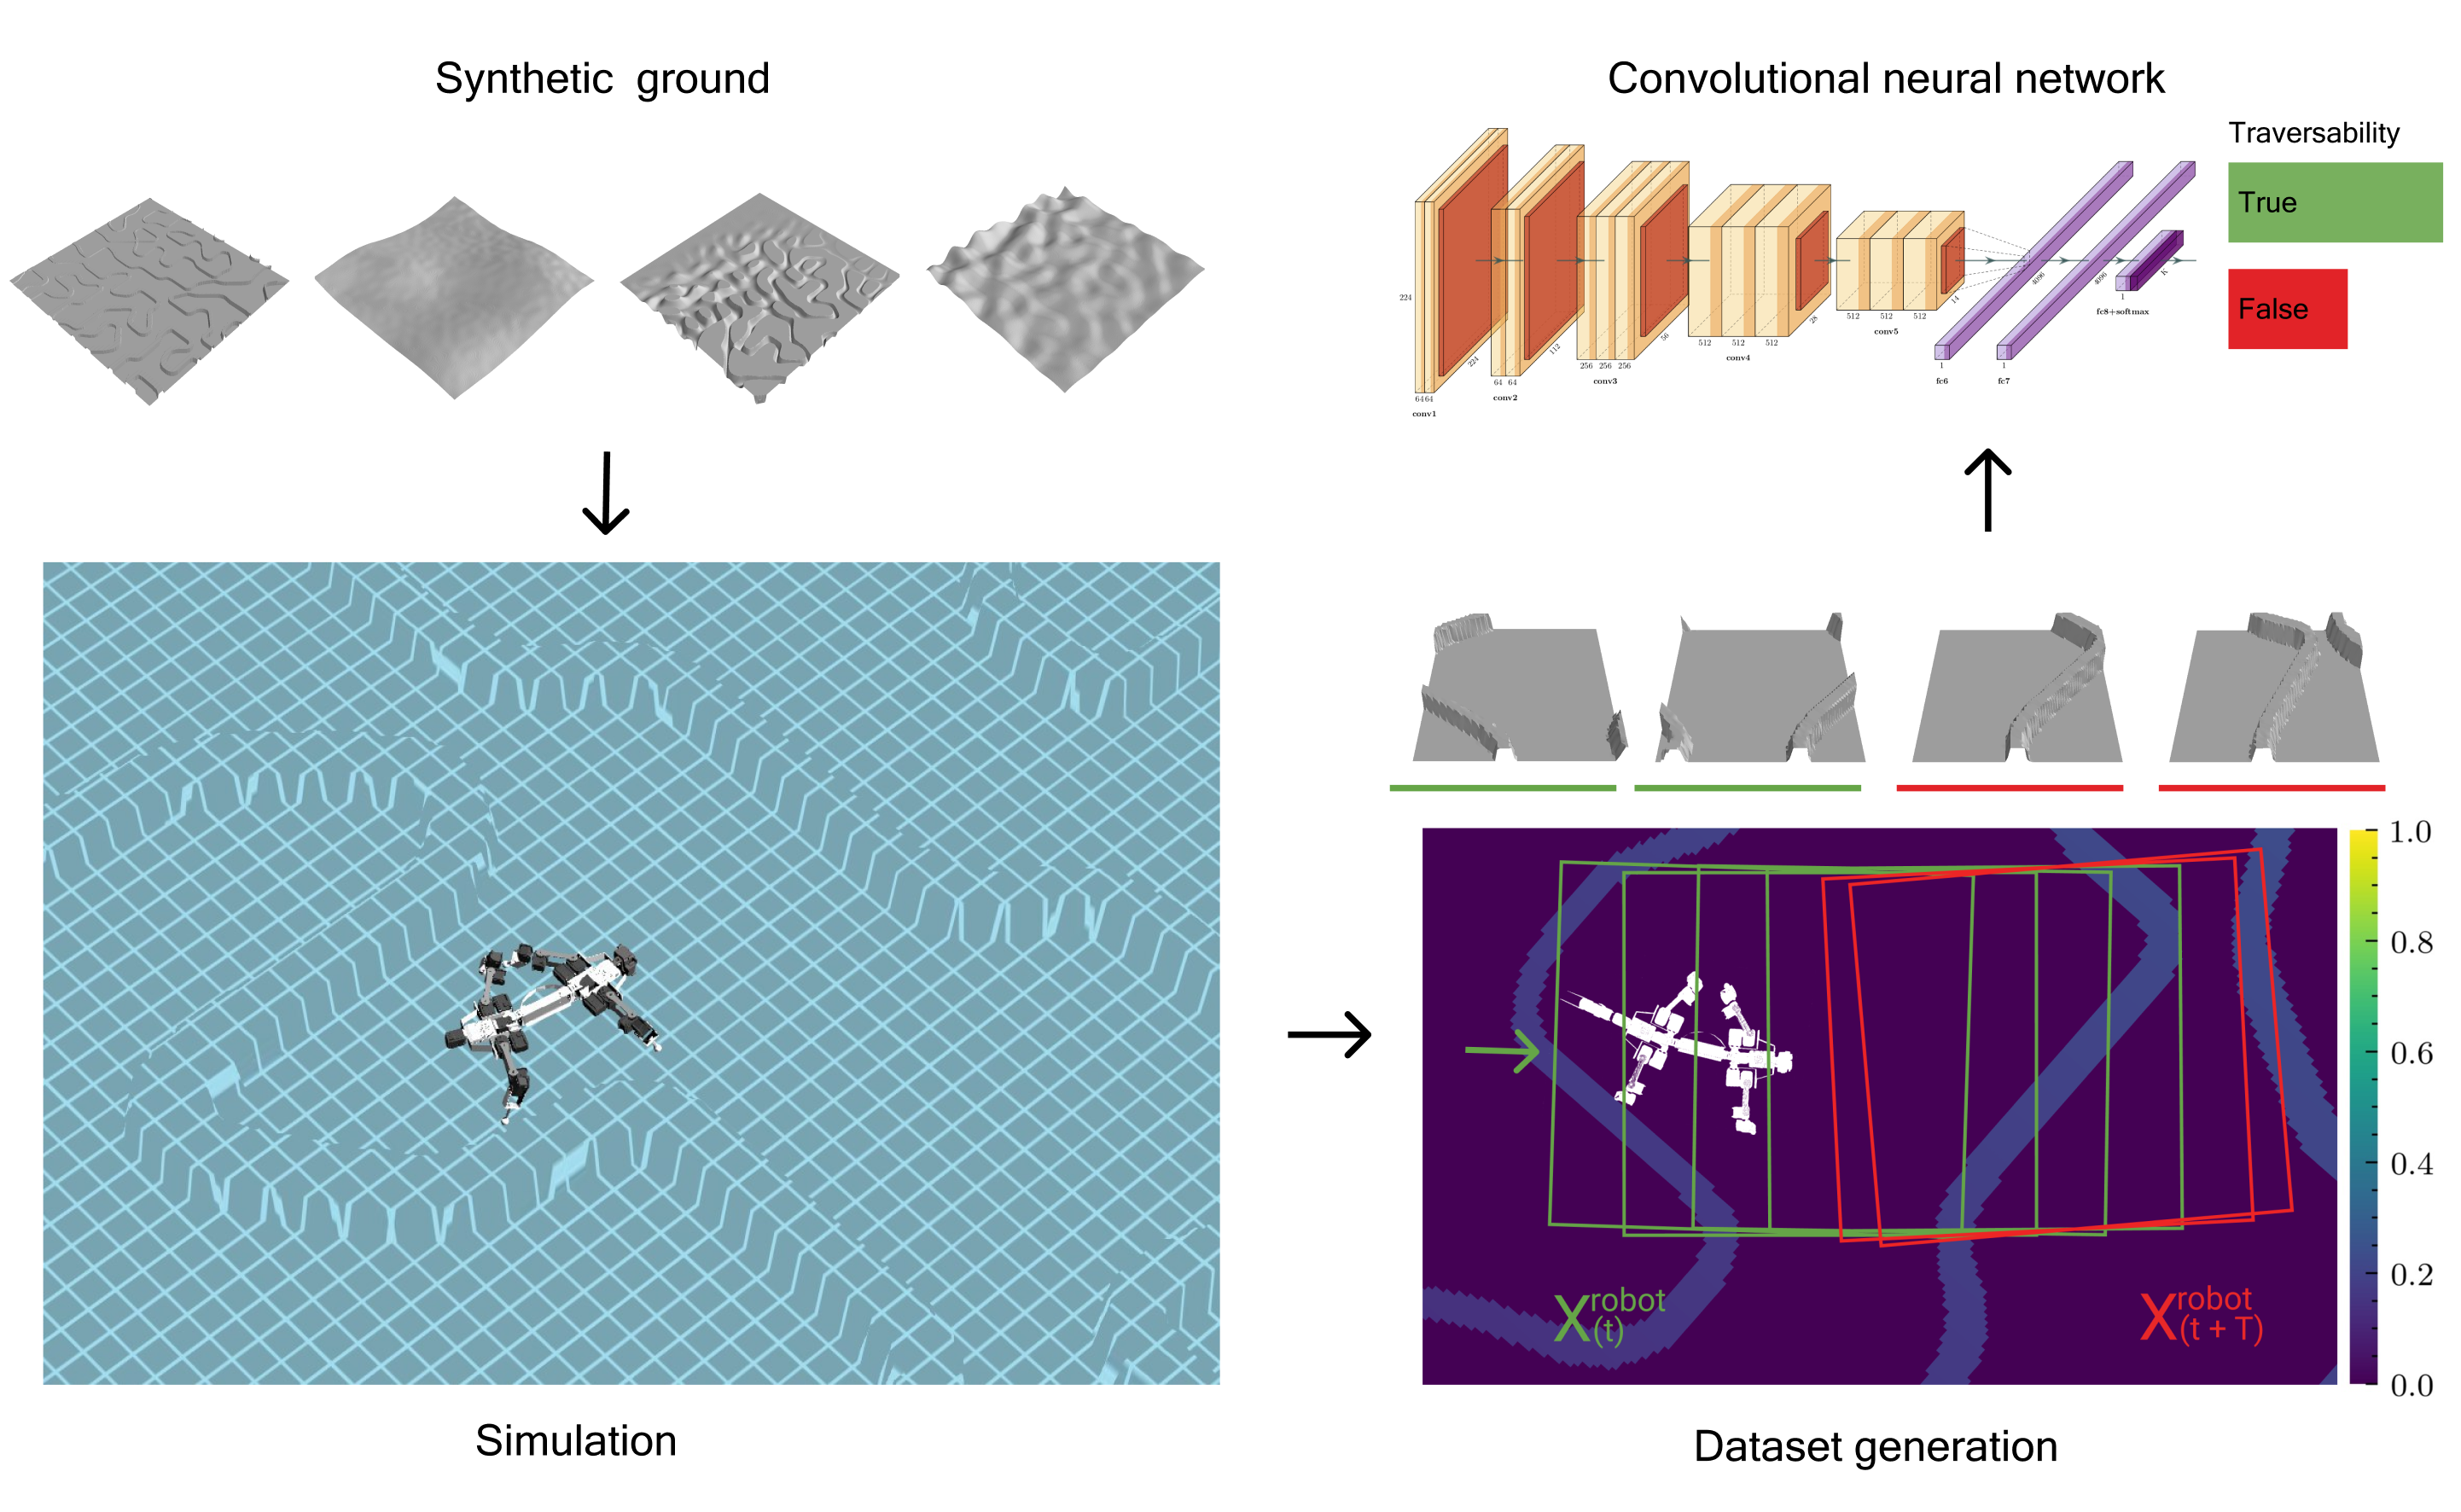
\includegraphics[width=\textwidth]{../img/method.png}
    \caption{The framework's main building block in counter-clockwise order. The robot is a legged robot crocodile-like. First, we generated meaningful synthetic grounds. Then, the robot randomly spawns and walks forward with a fix controller on the maps inside a simulated environment. While moving, it stores its interactions. Then, we crop a region of ground, a patch, for each simulation trajectory around the robot. The patch's size is calculated according to its locomotion. We labeled those images using a defined threshold. Finally, fit a deep convolutional neural network to predict traversability. }
    \label{fig : pipeline}
    \end{figure}
% advantanges
Collecting data through simulation has several main advantages such as variety, cost, and speed. With simulations, we can easily increase the number of data samples at any time by simply incorporate more maps or run more experiments. Contrarily, a real robot requires to first identify the suitable ground and then physically transport the machine there and finally let it walk on it. Also, real robots cannot completely explore all grounds due to the possibility to be damaged, especially in outdoors scenarios. This prevents the full exploration of the environment. On the other hand, a virtual robot can be destroyed and regenerate indefinitely. This allows a total exploration of all not traversable samples, essential to generate a quality dataset. Of course, a realistic model controller must be implemented to simulate the real robot.

Furthermore, we are not limited by real constraint and we can design the ground to maximize the variety of robot's interactions. For instance, we can artificial design maps to include any kind of situations and challenges.
Clearly, this also reduces the time required to collect the robot's interactions with the terrain. The time could be further minimized by running different simulations in parallel bypassing the demand for more physical hardware.
% data generation
To create a quality dataset, we must generate a series of various surfaces and ensure their diversity. Intuitively, those maps should be small enough to allow fast exploration but big enough to include several features. Modern ground made straightforward to generate a rich array of terrains with different characteristics such us bumps, ramps, slopes in different levels and sizes. There are several methods to represent terrain, we followed the generate procedure proposed in the original work \cite{omar2018traversability}.  Figure \ref{fig : grounds} shows a small collection of synthetic terrains with different features.
\begin{figure}[htbp]
    \centering
    \begin{subfigure}[b]{0.24\textwidth}
        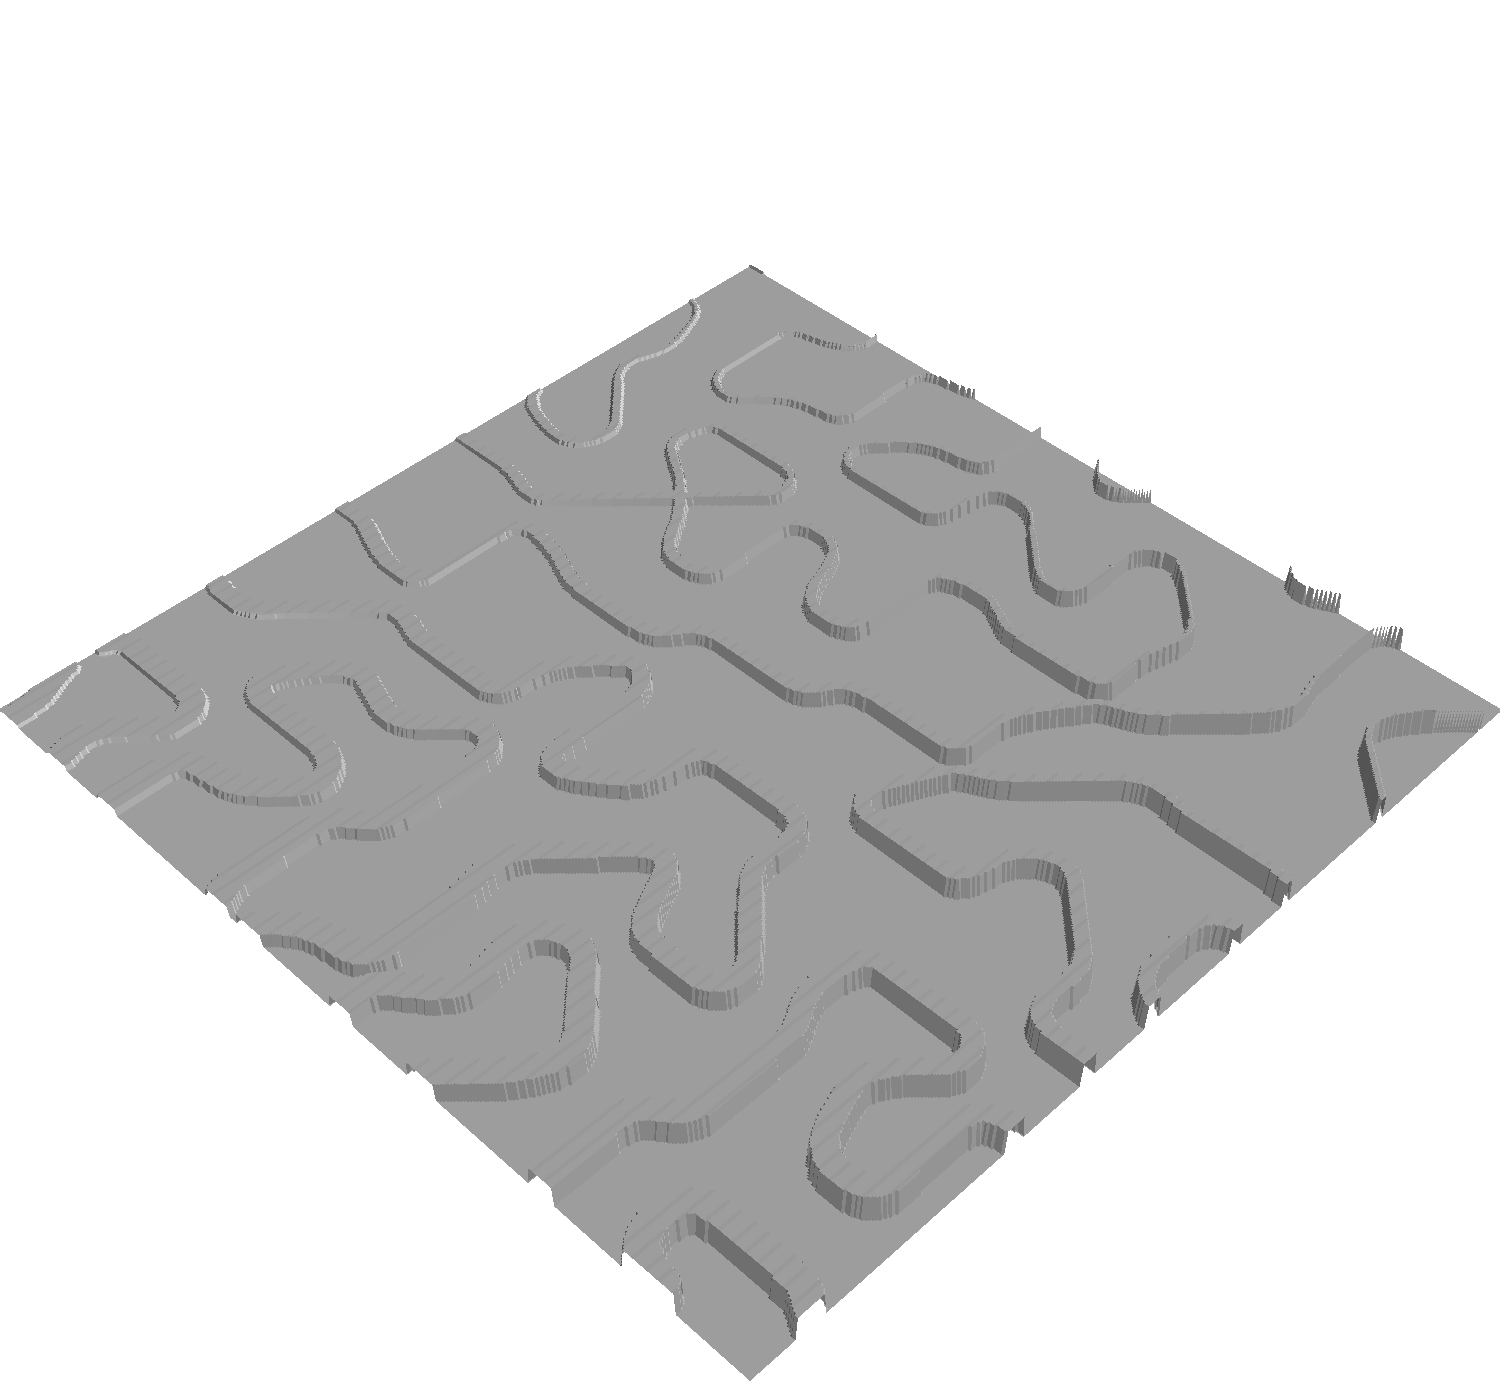
\includegraphics[width=\linewidth]{../img/hm3d/bars1.png}
        \caption{Walls.}
    \end{subfigure}
    \begin{subfigure}[b]{0.24\textwidth}
        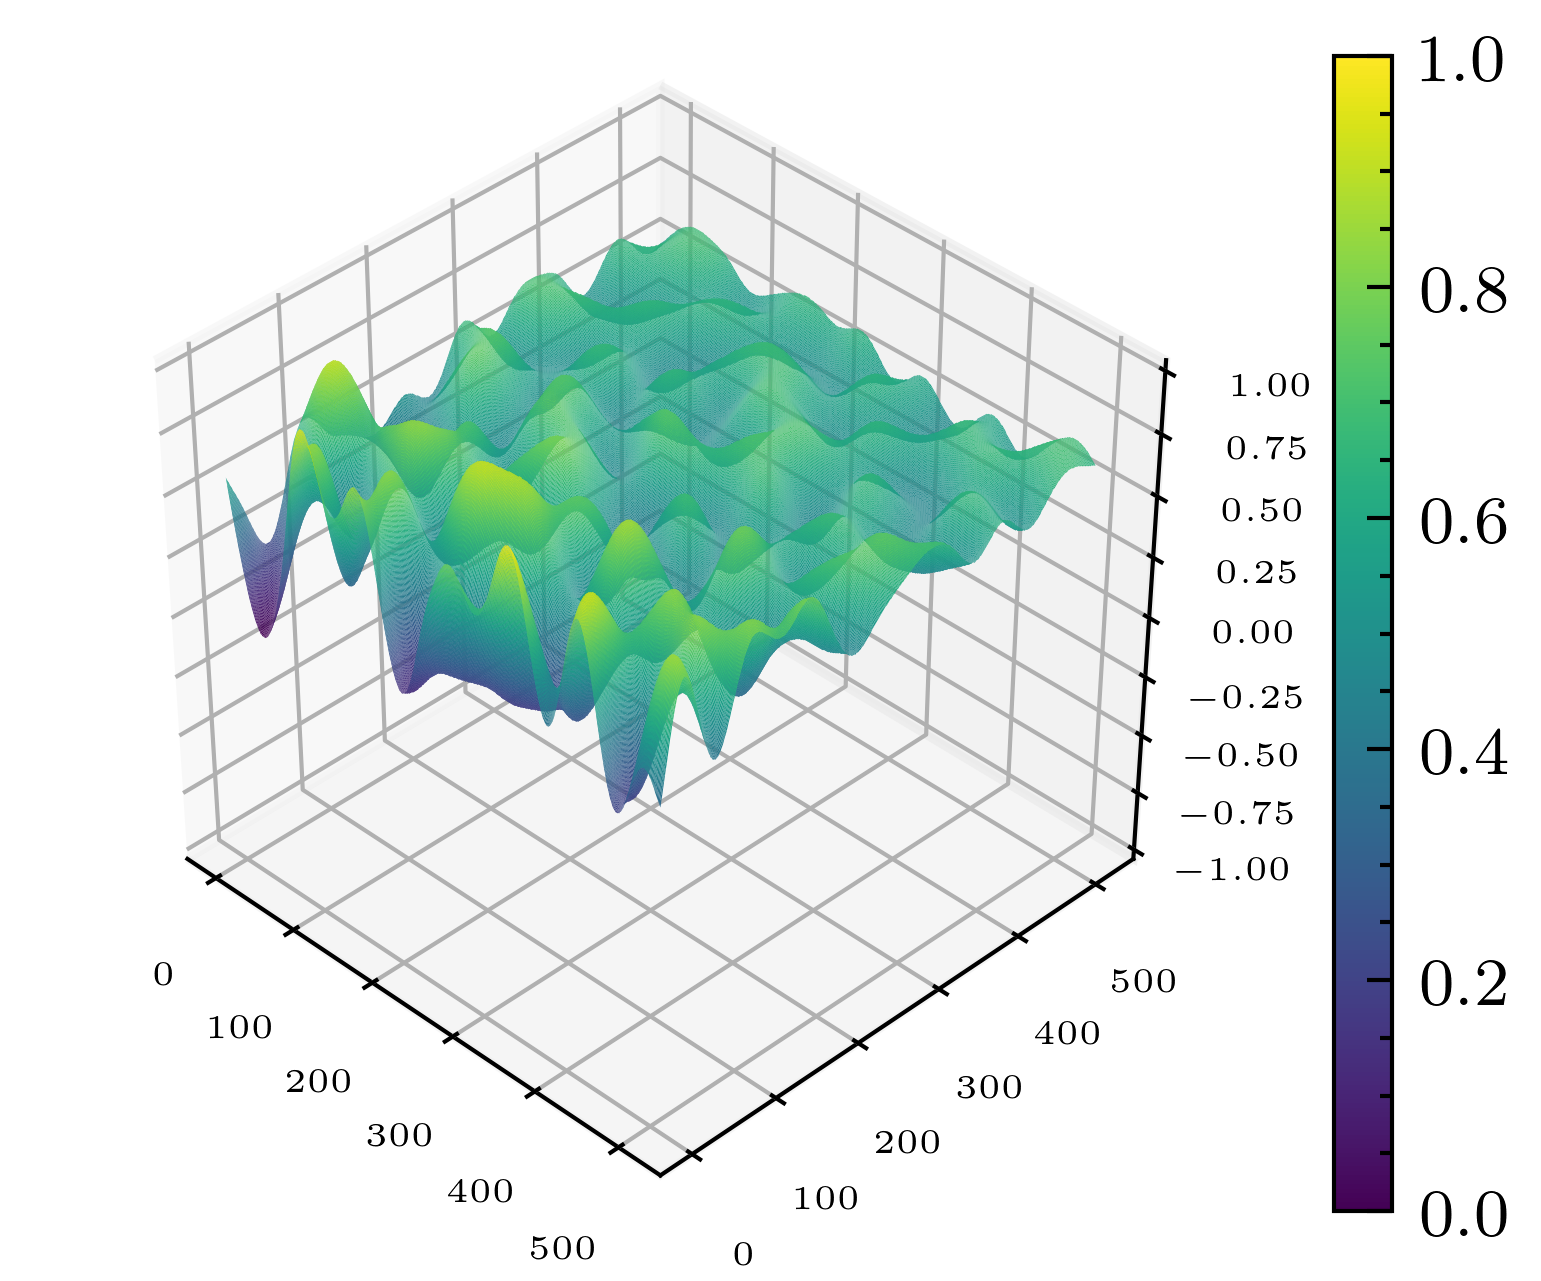
\includegraphics[width=\linewidth]{../img/hm3d/bumps2.png}
        \caption{Bumps.}
 \end{subfigure}  
    \begin{subfigure}[b]{0.24\textwidth}
        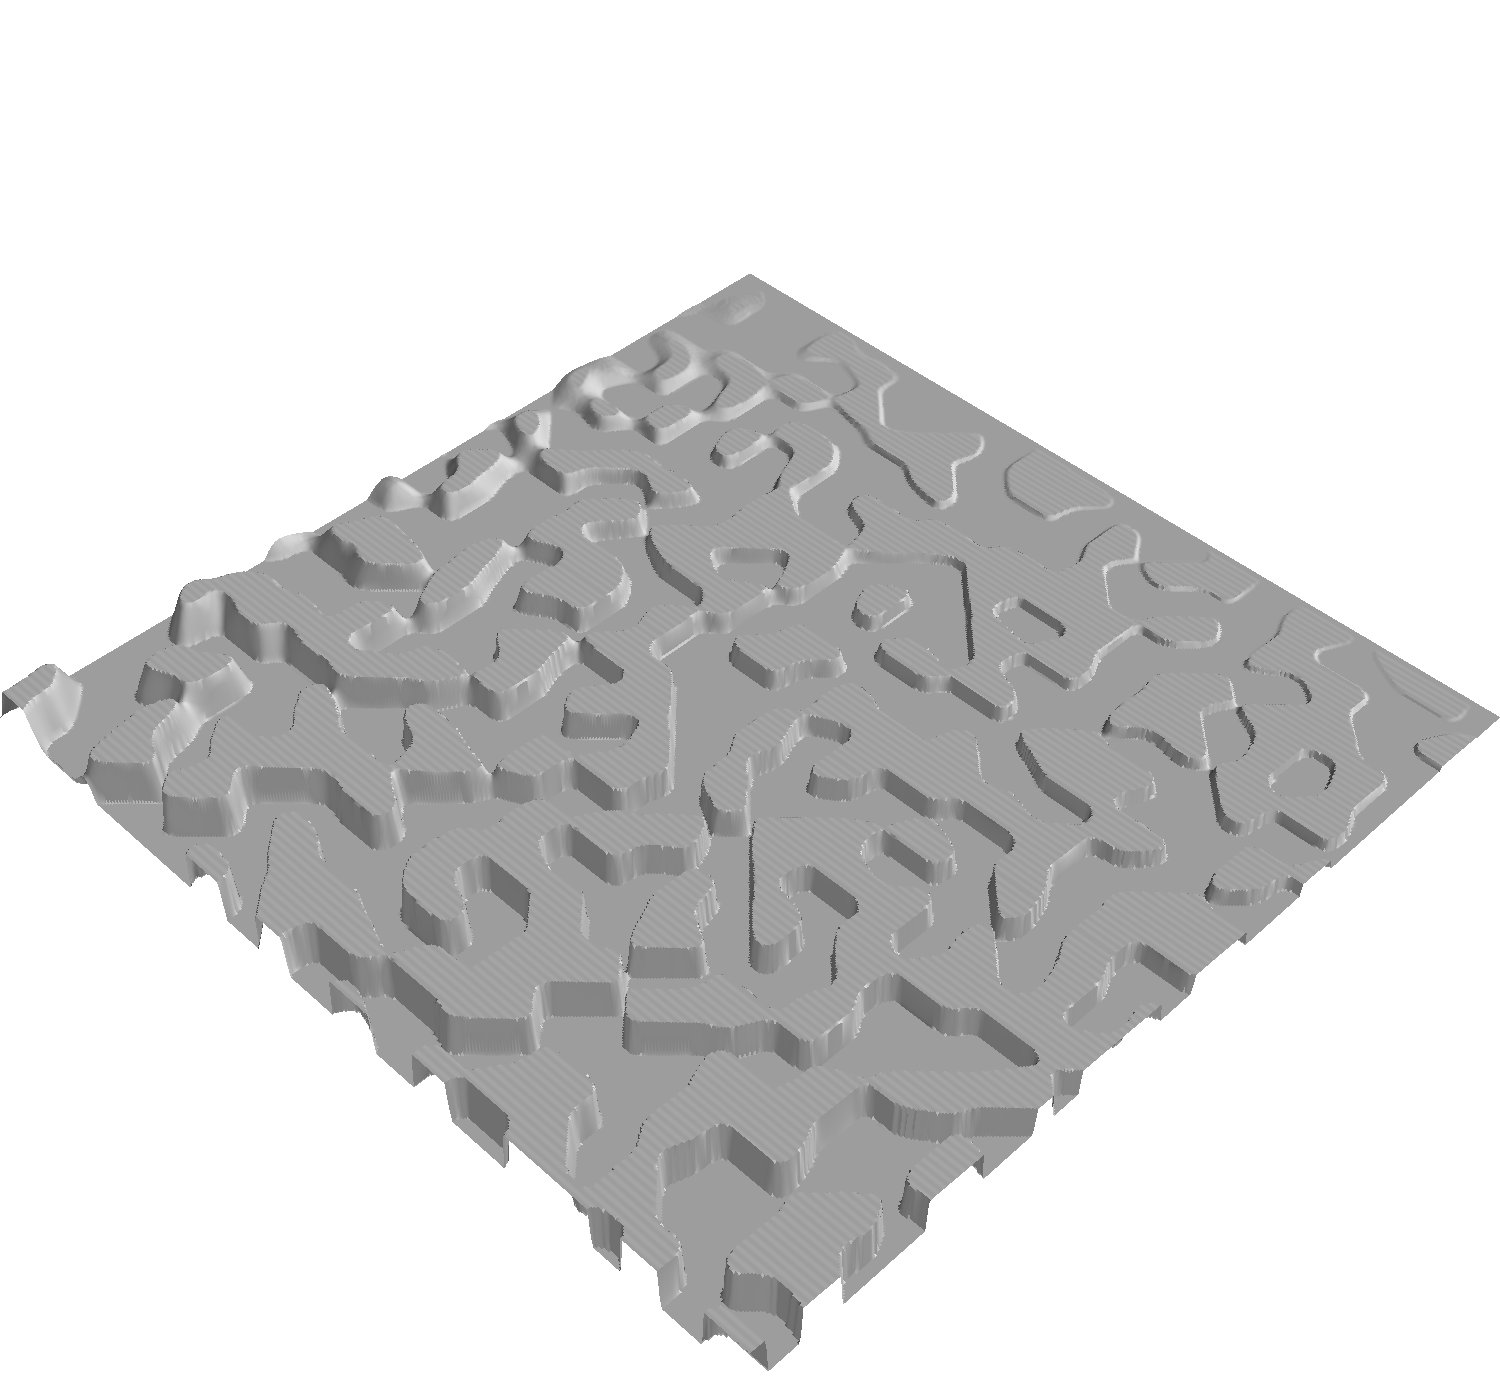
\includegraphics[width=\linewidth]{../img/hm3d/steps1.png}
        \caption{Steps.}
 \end{subfigure}  
    \begin{subfigure}[b]{0.24\textwidth}
        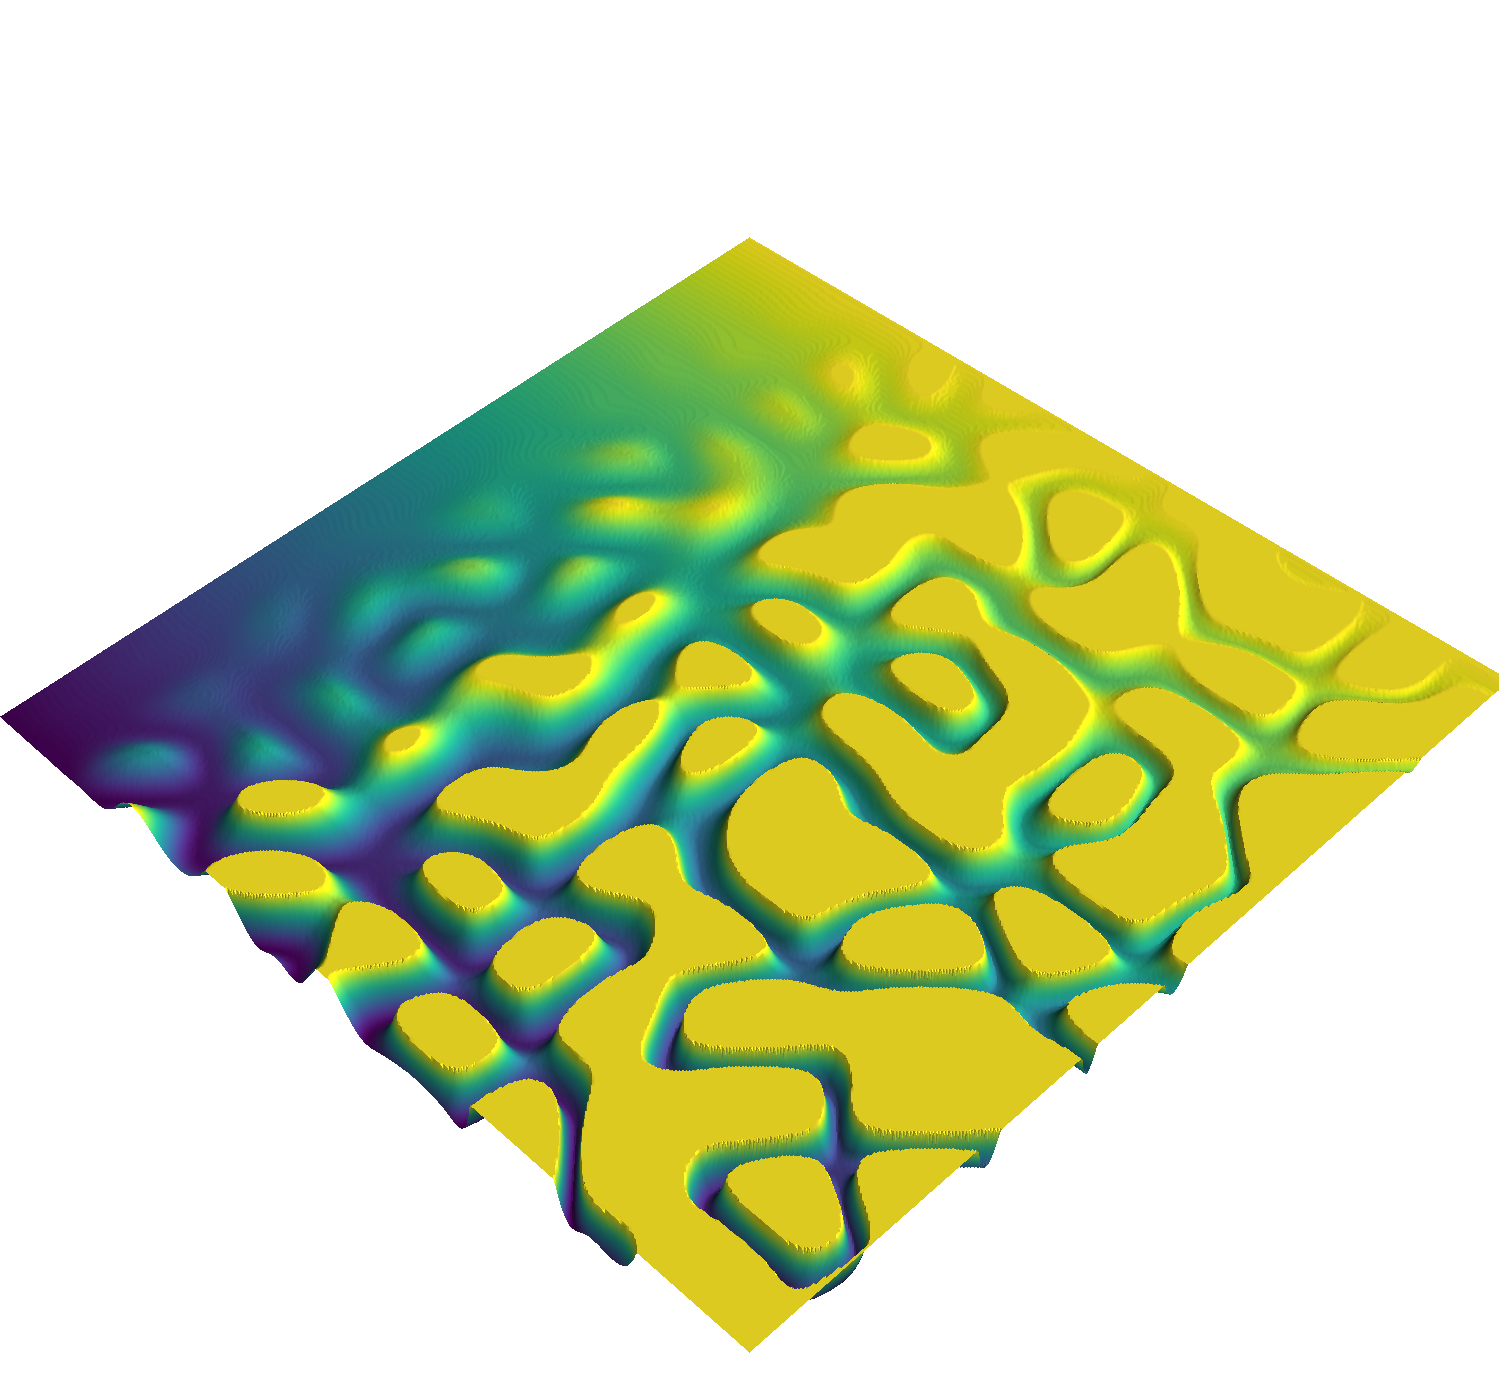
\includegraphics[width=\linewidth]{../img/hm3d/rails3.png}
        \caption{Rails.}
    \end{subfigure}  
\caption{Some artificially generated terrains, $10\times 10$m, with one specific feature each. }   
\label{fig : grounds}
\end{figure}
We represented the terrains with heightmaps, where the height component of the ground is stored as pixels in a gray image. Practically, the image is a top-view representation of the terrain where the brightness describes the height. 

Robots interacts with the maps when it is loaded on the simulator. To ensure a correct exploration of each terrain, we randomly spawn the robot multiple times on the same map and let it walk for a fixed amount of time. Random spawn reduces the possibility to repeatedly visiting the same spot and it maximizes the robot's exploration.

The robot position is tracked and stored during simulation to extract a small portion of ground, a patch, around each of its trajectory's position. The patches are cropped from the heightmap using a specific size based on the robot's footprint and its velocity. Each resulting image is labeled using a minimum advancement based on the robot's characteristic. We tested our framework on a legged crocodile-like robot called \emph{Krock}. Due to its four legs, the robot has very unique locomotion allowing it to overcome different obstacles making estimate traversability more challenging. Figure \ref{patch-extraction} helps to visualize the procedure. The dataset generation process is detailed explained in section \ref{sec: data-gathering}.  
\begin{figure} [htbp]
    \centering
    \begin{subfigure}[b]{0.66\textwidth}
    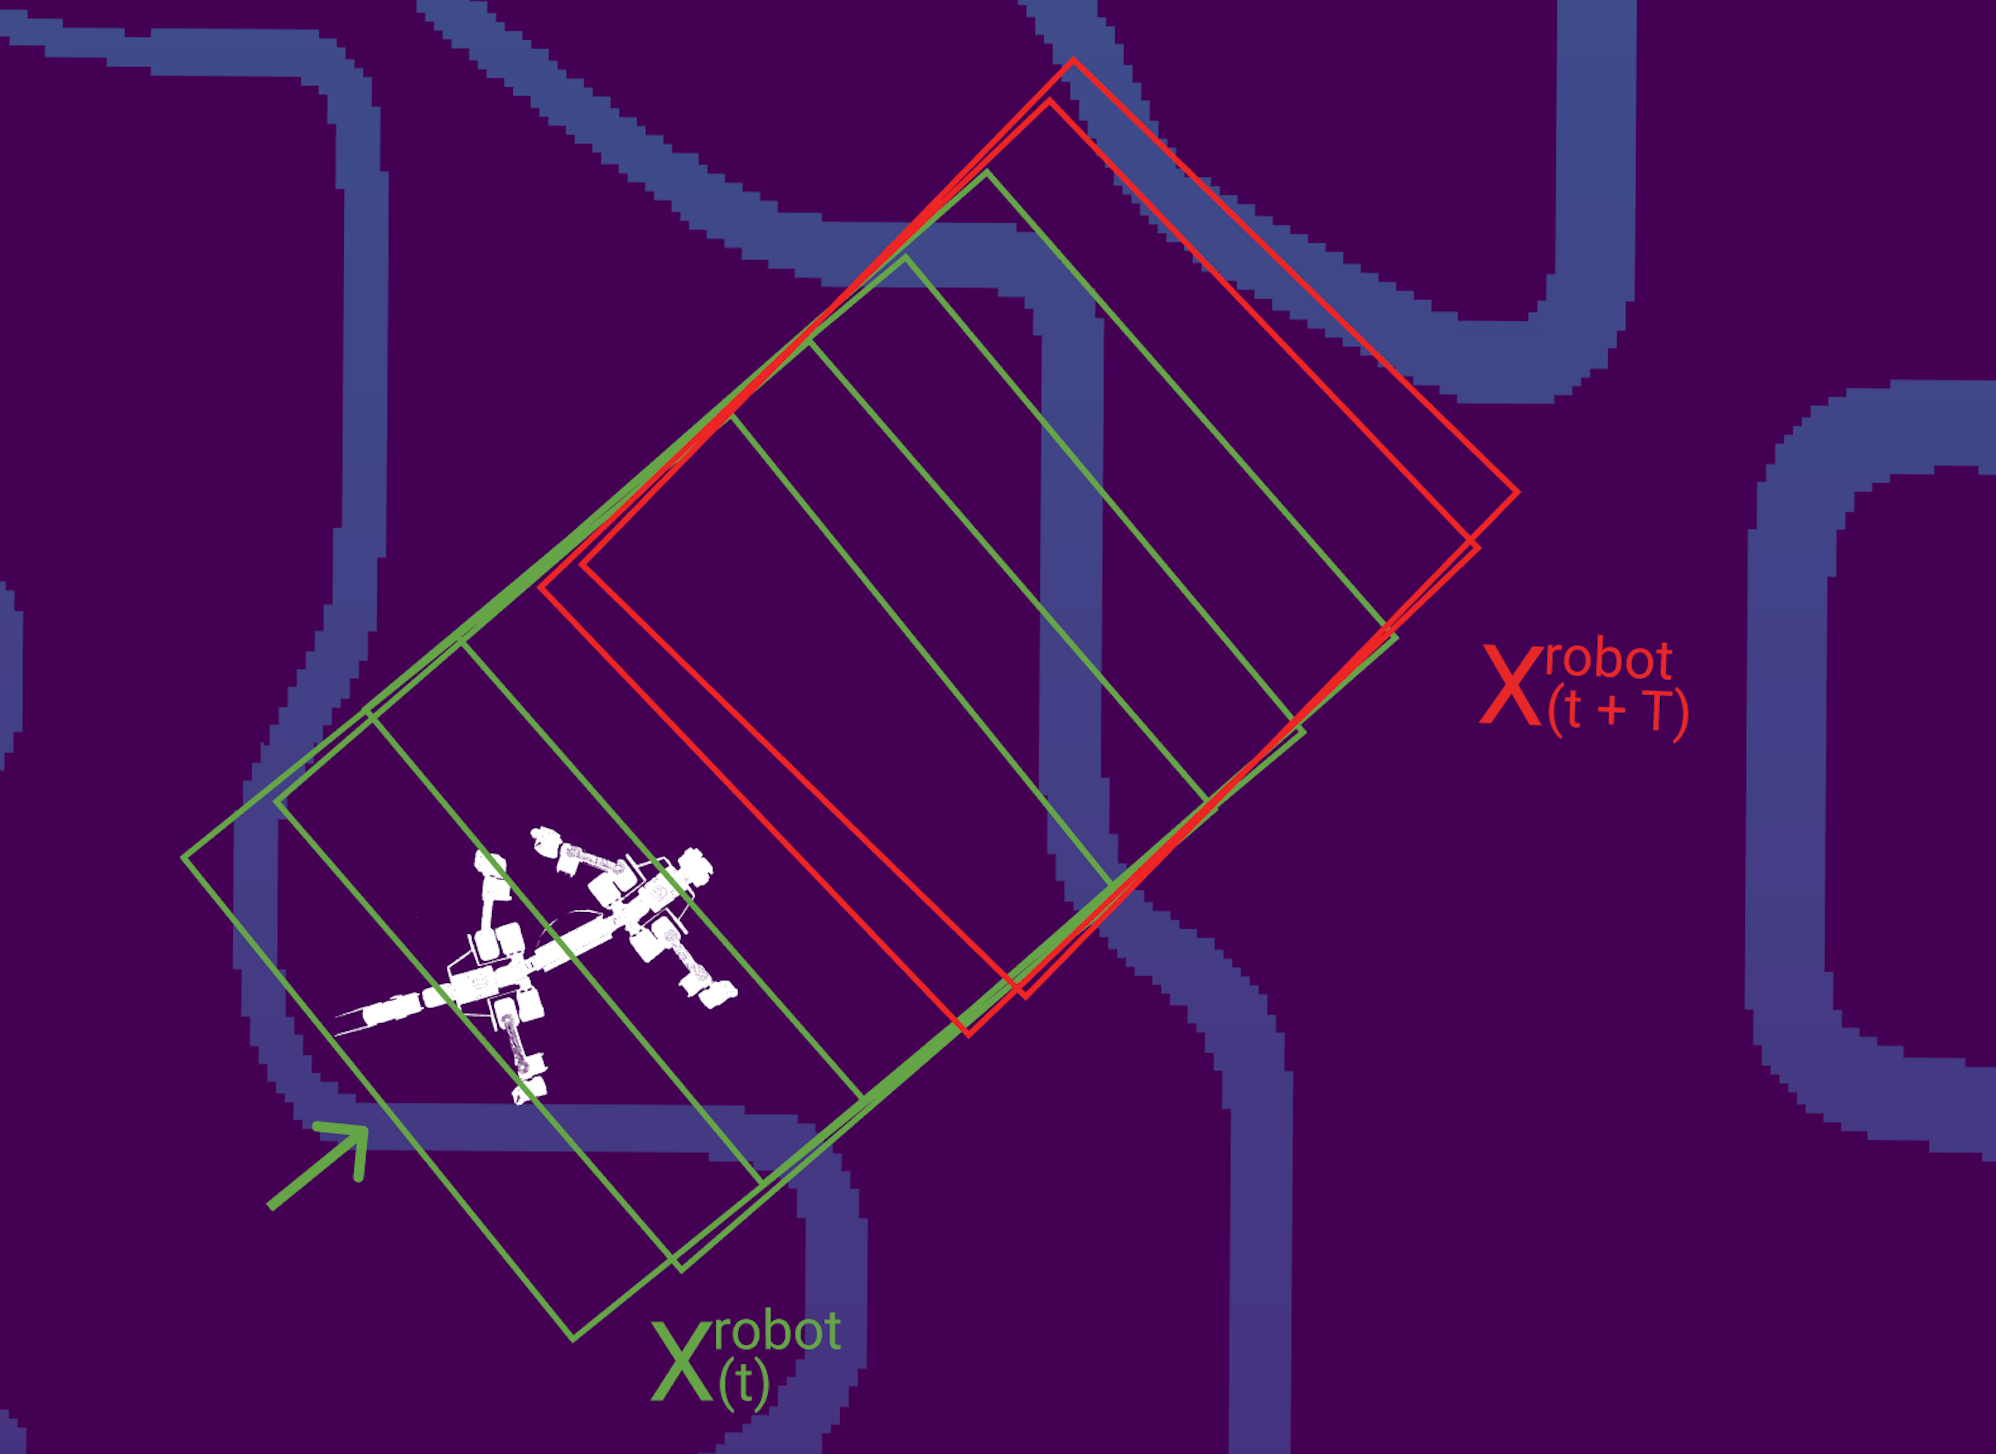
\includegraphics[width=\textwidth]{../img/krock-bars-correct-small.png}
    \caption{Robot's trajectory.}
\end{subfigure}
\begin{subfigure}[b]{1\textwidth}
    \begin{subfigure}[b]{0.24\textwidth}
    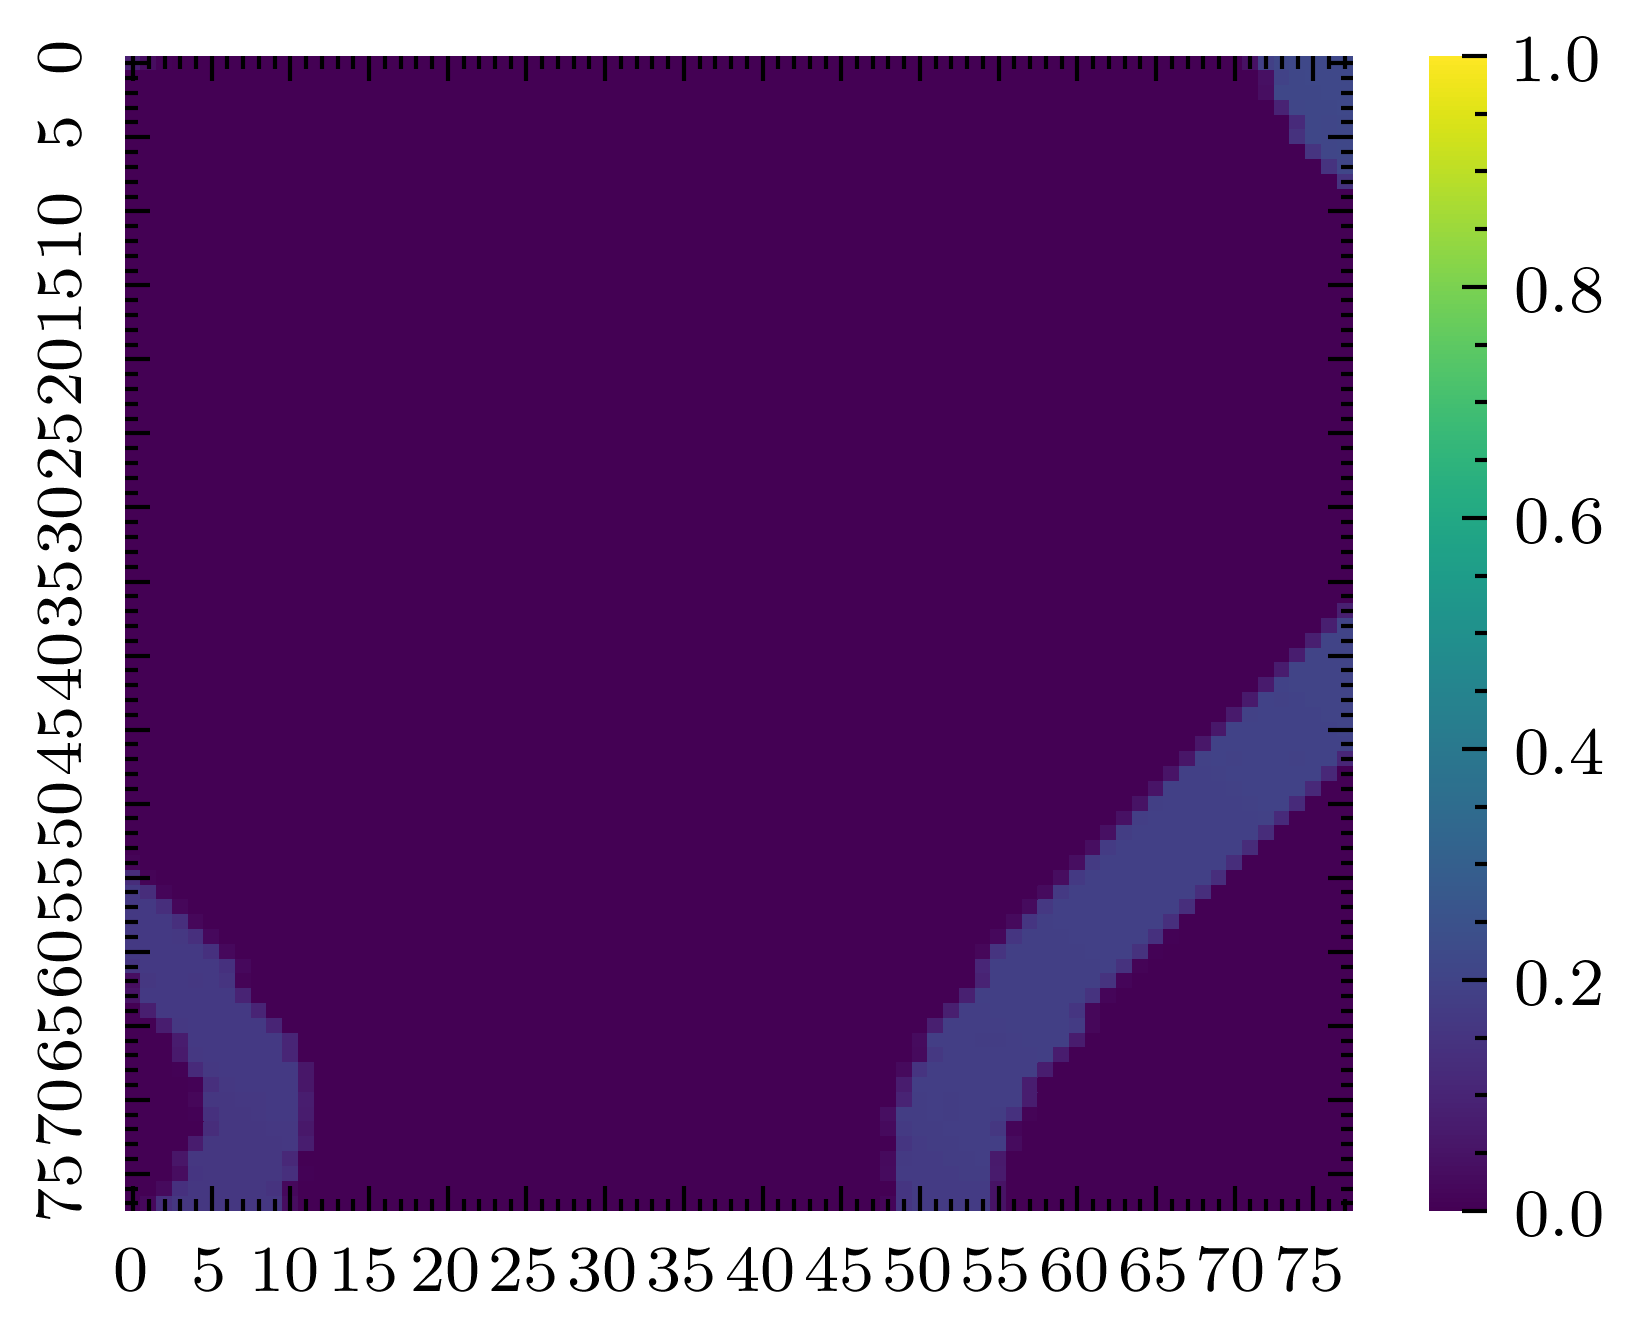
\includegraphics[width=\linewidth]{../img/bars1-example-patches/2d/2.png}    
    \end{subfigure}  
    \begin{subfigure}[b]{0.24\textwidth}
    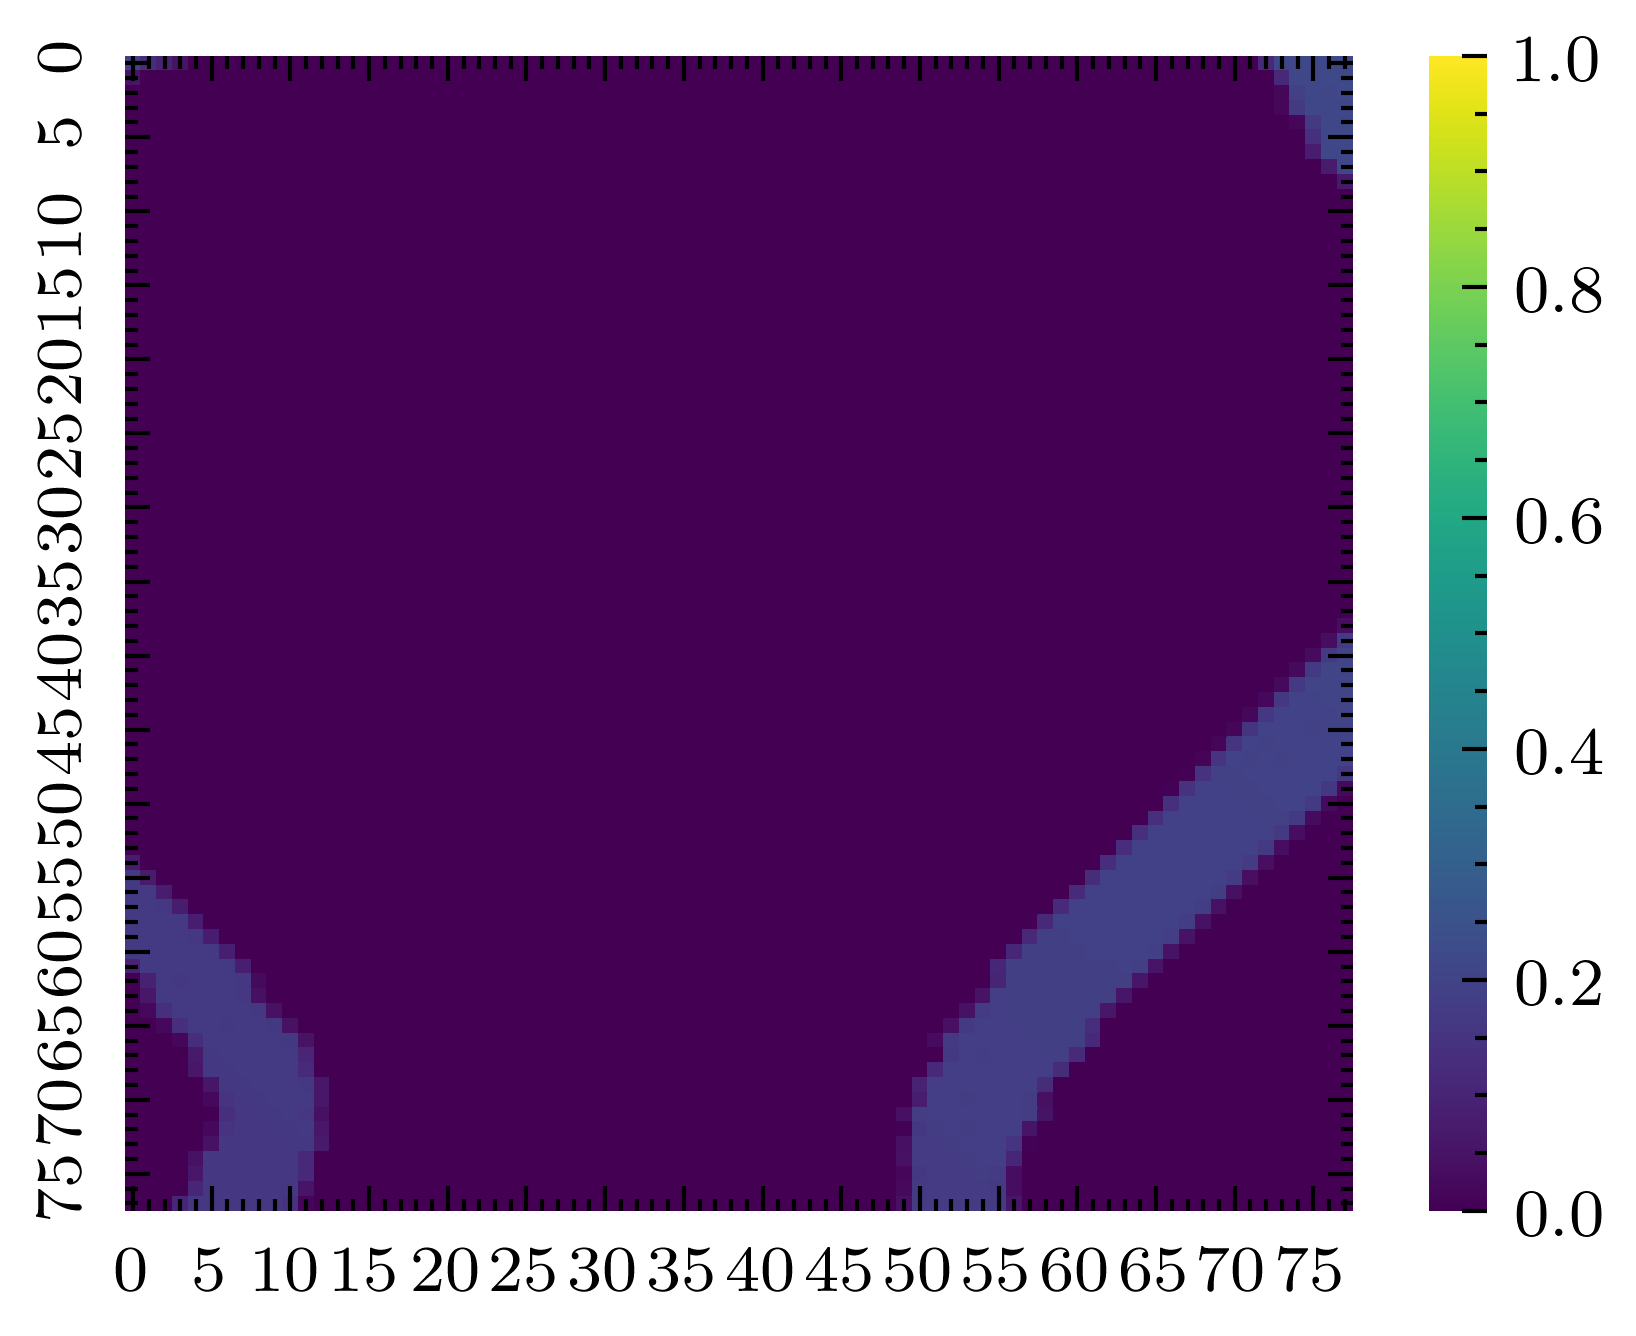
\includegraphics[width=\linewidth]{../img/bars1-example-patches/2d/4.png} 
    \end{subfigure}
    \begin{subfigure}[b]{0.24\textwidth}
    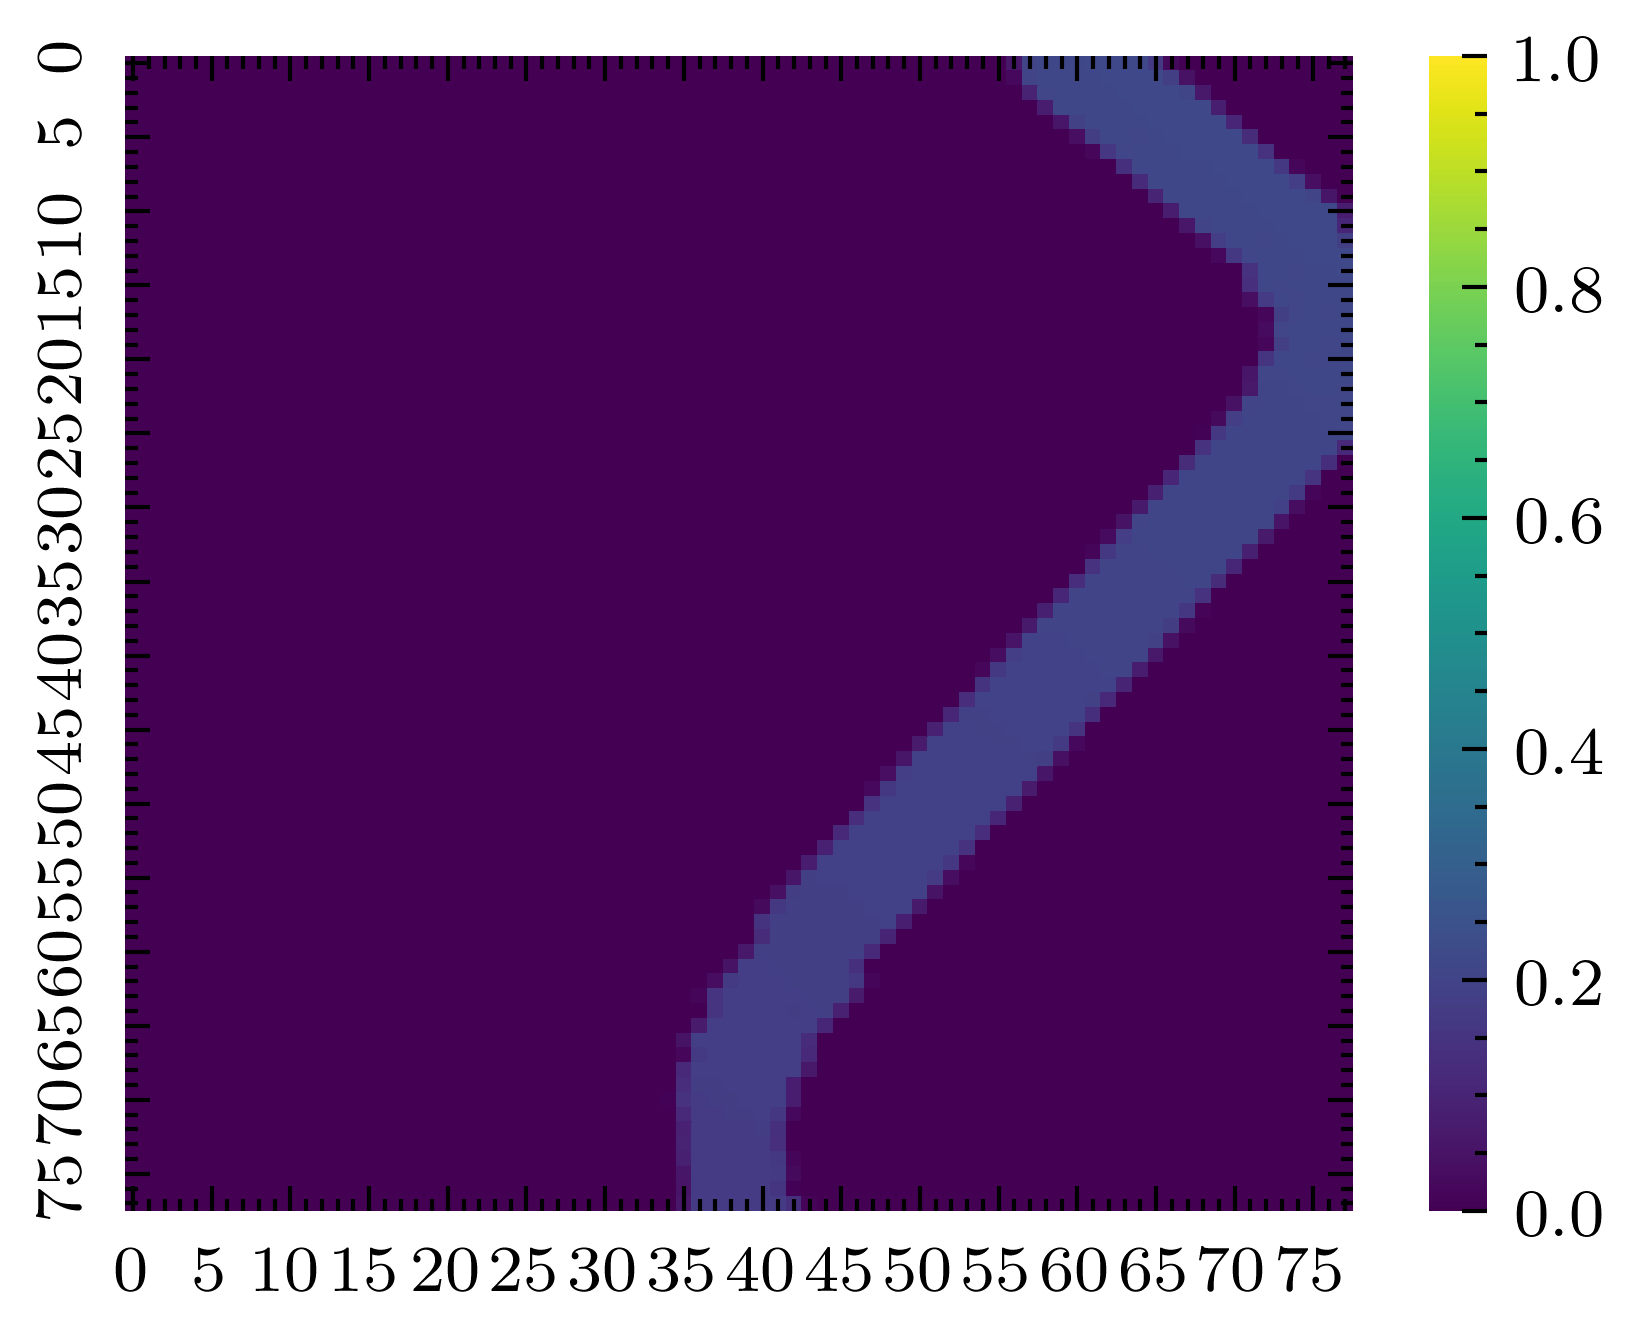
\includegraphics[width=\linewidth]{../img/bars1-example-patches/2d/7.png}    
    \end{subfigure}  
    \begin{subfigure}[b]{0.24\textwidth}
    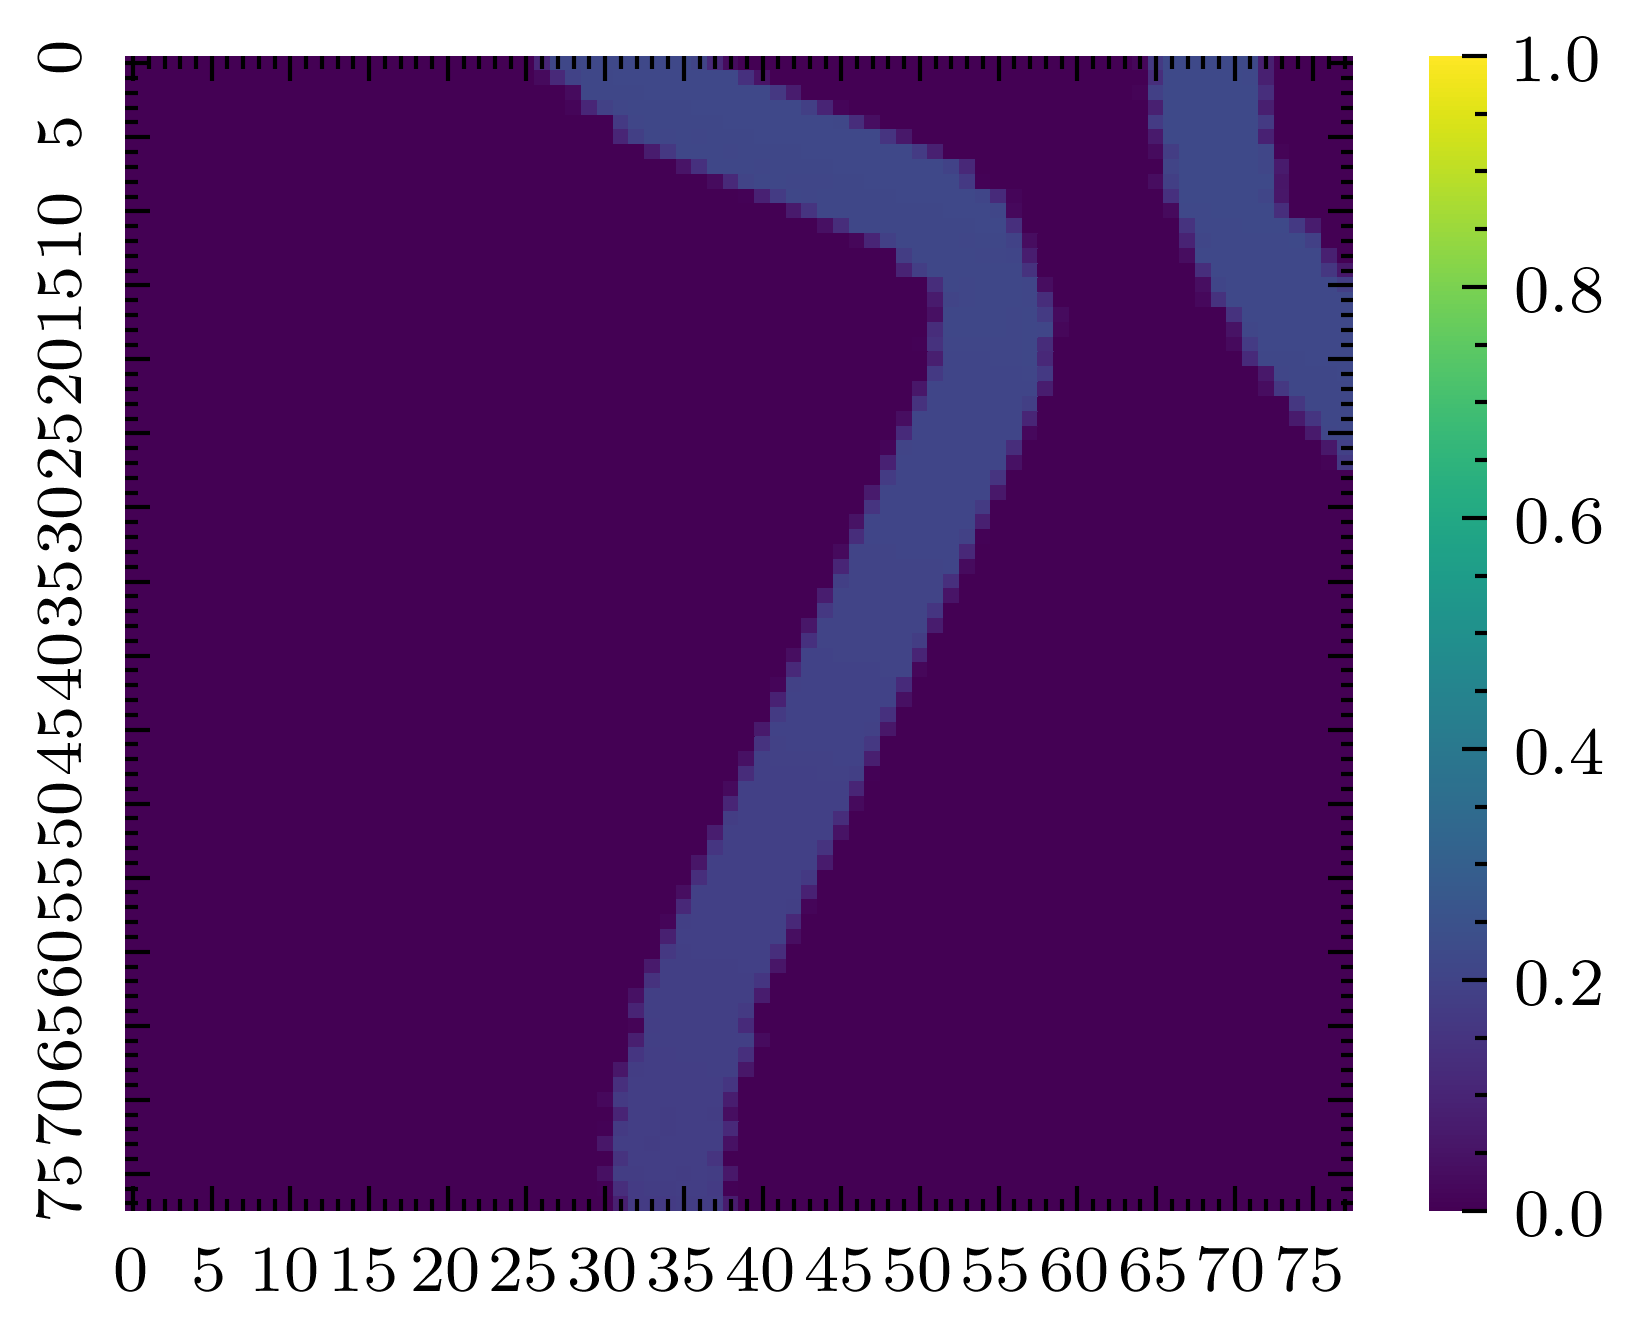
\includegraphics[width=\linewidth]{../img/bars1-example-patches/2d/14.png}    
    \end{subfigure}  
\caption{2D patches topview representation.}
\end{subfigure}  
\begin{subfigure}[b]{1\textwidth}
    \begin{subfigure}[b]{0.24\textwidth}
    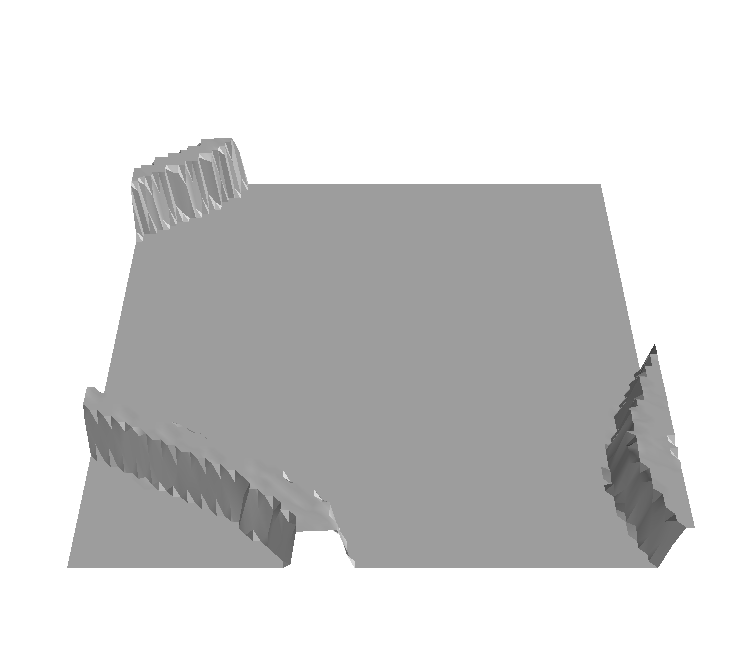
\includegraphics[width=\linewidth]{../img/bars1-example-patches/3d/2.png}    
    \end{subfigure}  
    \begin{subfigure}[b]{0.24\textwidth}
    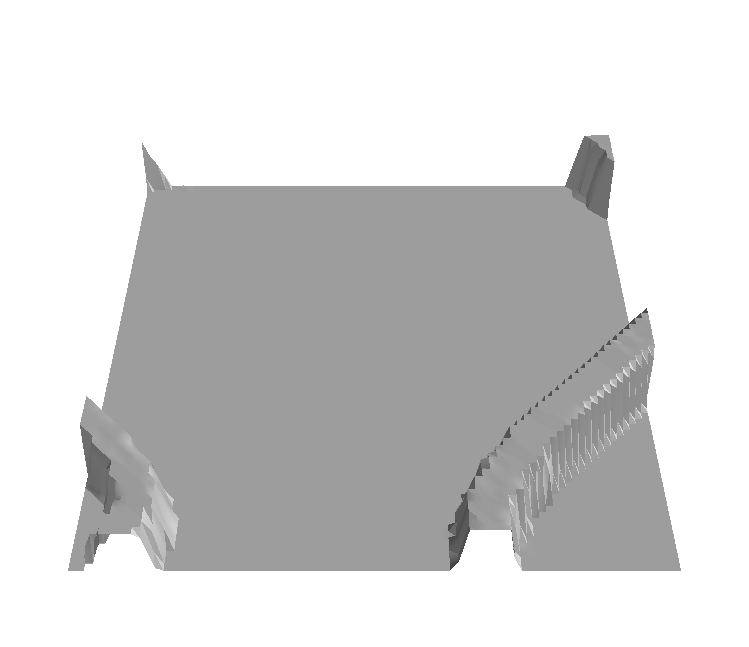
\includegraphics[width=\linewidth]{../img/bars1-example-patches/3d/4.png} 
    \end{subfigure}
    \begin{subfigure}[b]{0.24\textwidth}
    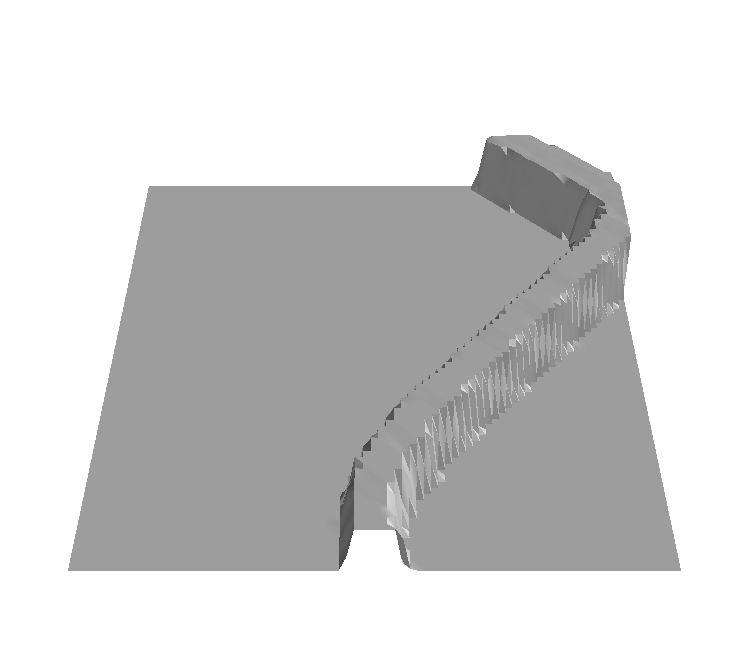
\includegraphics[width=\linewidth]{../img/bars1-example-patches/3d/7.png}    
    \end{subfigure}  
    \begin{subfigure}[b]{0.24\textwidth}
    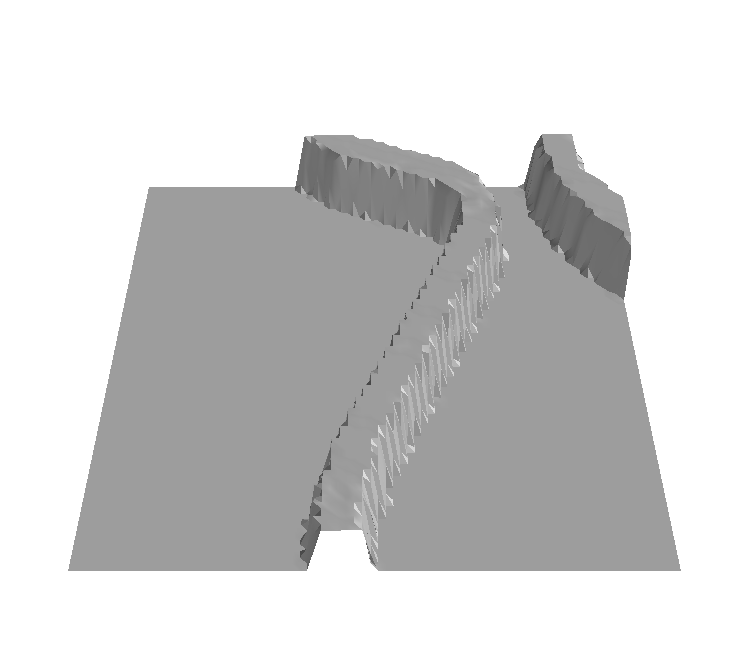
\includegraphics[width=\linewidth]{../img/bars1-example-patches/3d/14.png}    
    \end{subfigure}  
\caption{3D patches representation.}
\label{fig : patch-extraction}
\end{subfigure}
\caption{Example of a robot's trajectory (a) extracted during training on a map with different walls. Robot's initial position is shown by its white silhouette. Patches borders are labeled with greed if traversable and red if not and showed as 2D (b) and 3D(c) rendered images. The robot traverses the patches from left to right.}
\end{figure}

The dataset generated is fed to a deep convolutional neural network. The model estimates traversability given an heightmap, an image, representing a small region of terrain as input. We improved the original architecture by adopting a ResNet variant based on recent works \cite{he2015deep} \cite{he2015identity} \cite{hu2017squeeze}. We methodologically tested different variant of the new architecture to finally generate a model with three-time fewer parameters than the original network, comparable performance. Due to its smaller size, the network has a lower prediction time than the original one. Thus, it is can be deployed easier using less demanding hardware . We appraised the models' performance booth quantitatively, with numerical metrics, and qualitatively, showing the traversability estimation on real-world terrains.

In chapter \ref{chap: interpretability}, we test the model's predictions robustness using different techniques. First, we proved the network's ability to learn meaningful features from the inputs, section \ref{sec:  features-separability}. Then, \ref{sec: quarry-dataset} we visualize different inputs to understand which grounds' regions caused the predictions.  We adopted a technique that allows highlighting the part of the terrain contributes the most to the network's output. Lastly, in section \ref{sec: robustness}, we tested the model's robustness by creating different patches with unique characteristics. We compared the estimator's predictions to the ground truth gather the simulator.

% To summarize our contributions to literature are the implementation of a framework to learn traversability entirely through simulation that can be employed with any mobile robot, a new small neural network architecture able to reach high accuracy, different real-world evaluations, and a model interpretability case study to understand the strengths and limitations of the trained model. 

\end{document}
